\documentclass[12pt,a4paper]{article}
\usepackage[utf8]{inputenc}
\usepackage[vietnamese]{babel}
\usepackage{graphicx}
\usepackage{float}
\usepackage{geometry}
\geometry{a4paper, margin=2.5cm}
\usepackage{hyperref}
\usepackage{xcolor}
\usepackage{fancyhdr}
\usepackage{titlesec}
\usepackage{booktabs}
\usepackage{array}

\hypersetup{
    colorlinks=true,
    linkcolor=blue,
    filecolor=magenta,      
    urlcolor=cyan,
    pdftitle={Bao cao Bai tap 4 - Cong cu hop tac truc tuyen},
    pdfpagemode=FullScreen,
}

% Cấu hình header & footer
\pagestyle{fancy}
\fancyhf{}
\rhead{Hành trình Kỹ năng số}
\lhead{Bài tập Thực hành 4}
\rfoot{Trang \thepage}

% Định dạng tiêu đề mục
\titleformat{\section}{\normalfont\Large\bfseries\color{blue!80!black}}{\thesection}{1em}{}
\titleformat{\subsection}{\normalfont\large\bfseries\color{blue!60!black}}{\thesubsection}{1em}{}

\begin{document}

% --- TRANG BÌA ---
\begin{titlepage}
    \centering
    \vspace*{1cm}
    
    {\large \bfseries TRƯỜNG ĐẠI HỌC CÔNG NGHỆ - ĐHQGHN} \\[0.2cm]
    {\large \bfseries KHOA CÔNG NGHỆ THÔNG TIN} \\[1.5cm]
    
    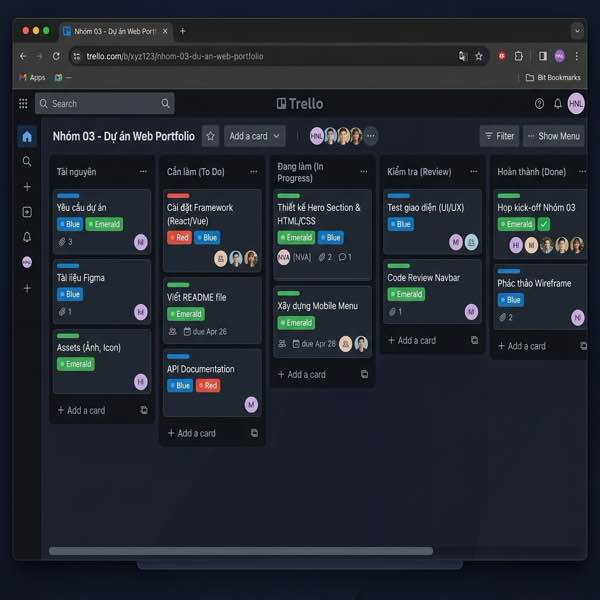
\includegraphics[width=0.3\textwidth]{images/trello_board.jpg} \\[1.5cm]
    
    {\Large \bfseries BÁO CÁO BÀI TỰ THỰC HÀNH CÁ NHÂN} \\[0.5cm]
    {\Huge \bfseries BÀI TẬP 4: SỬ DỤNG CÔNG CỤ HỢP TÁC TRỰC TUYẾN TRONG DỰ ÁN NHÓM} \\[1.5cm]
    
    \textbf{Môn học:} Nhập môn Công nghệ số và Ứng dụng Trí tuệ nhân tạo \\
    \textbf{Chủ đề:} Quản lý tác vụ, Giao tiếp và Lưu trữ tài nguyên cộng tác \\[2cm{}]
    
    \begin{flushleft}
        \large
        \textbf{Sinh viên thực hiện:} Nguyễn Bảo Đăng \\
        \textbf{Mã số sinh viên:} 25020115 \\
        \textbf{Lớp học:} 23\_1 \\
        \textbf{Giảng viên hướng dẫn:} PGS. TS. Nguyễn Văn B
    \end{flushleft}
    
    \vfill
    {\large Thành phố Hồ Chí Minh, năm 2026}
\end{titlepage}

\newpage
\tableofcontents
\newpage

% --- NỘI DUNG CHÍNH ---

\section{Giới thiệu Dự án và Vai trò cá nhân}

\subsection{Bối cảnh dự án nhóm}
Trong khuôn khổ môn học "Nhập môn Công nghệ số và Ứng dụng Trí tuệ nhân tạo", nhóm 03 gồm 4 thành viên đã thực hiện một dự án nhỏ phát triển website Landing Page giới thiệu sản phẩm phần mềm (Website Redesign Project). Để thực hiện dự án này một cách hiệu quả trong thời gian ngắn (1 tuần), nhóm đã áp dụng các công cụ hợp tác trực tuyến để điều phối công việc từ xa, đảm bảo tiến độ và chất lượng sản phẩm.

\subsection{Vai trò và nhiệm vụ cá nhân}
Trong dự án này, tôi (\textbf{Nguyễn Bảo Đăng}) đảm nhận vai trò \textbf{Front-end Developer chính}. Các nhiệm vụ cá nhân do tôi phụ trách trong suốt tuần dự án bao gồm:
\begin{itemize}
    \item Thiết kế wireframe cấu trúc và xây dựng mã nguồn HTML/CSS cho trang chủ (đặc biệt là Hero Section).
    \item Tạo các hiệu ứng chuyển động và tương tác hover trên nút bấm bằng JavaScript.
    \item Phối hợp viết bản thảo đề xuất dự án trên tài liệu chung.
    \item Tổ chức lưu trữ toàn bộ mã nguồn tĩnh và tài nguyên thiết kế (hình ảnh, biểu tượng) của dự án.
\end{itemize}

\subsection{Danh sách các công cụ trực tuyến sử dụng}
Để tối ưu hóa không gian làm việc trực tuyến, cá nhân tôi đã tham gia thiết lập và sử dụng 4 công cụ thuộc các nhóm tính năng khác nhau:
\begin{enumerate}
    \item \textbf{Trello} (Quản lý dự án \& Tác vụ cá nhân)
    \item \textbf{Slack} (Giao tiếp nhóm \& Hỗ trợ kỹ thuật)
    \item \textbf{Google Docs} (Soạn thảo văn bản và đề xuất dự án cộng tác)
    \item \textbf{Google Drive} (Lưu trữ và phân quyền chia sẻ tài nguyên)
\end{enumerate}

\newpage
\section{Thiết lập Không gian làm việc và Nhật ký minh chứng}
Để đạt điểm tối đa theo tiêu chuẩn đánh giá, dưới đây là nhật ký hoạt động chi tiết cùng 9 hình ảnh minh chứng sắc nét thể hiện rõ tên tài khoản và phần đóng góp thực tế của tôi.

\subsection{Quản lý tác vụ cá nhân trên Trello}
Không gian Trello của Nhóm 03 được cấu trúc thành các danh sách: \textit{Tài nguyên, Cần làm, Đang làm, Kiểm tra, Hoàn thành}. Tôi đã sử dụng các nhãn màu (Labels) như đỏ (High Priority), xanh lá (Emerald) để gắn mức độ ưu tiên, đặt thời hạn cụ thể (due date) và thêm danh sách công việc con (Checklist) cho thẻ của mình.

\begin{figure}[H]
    \centering
    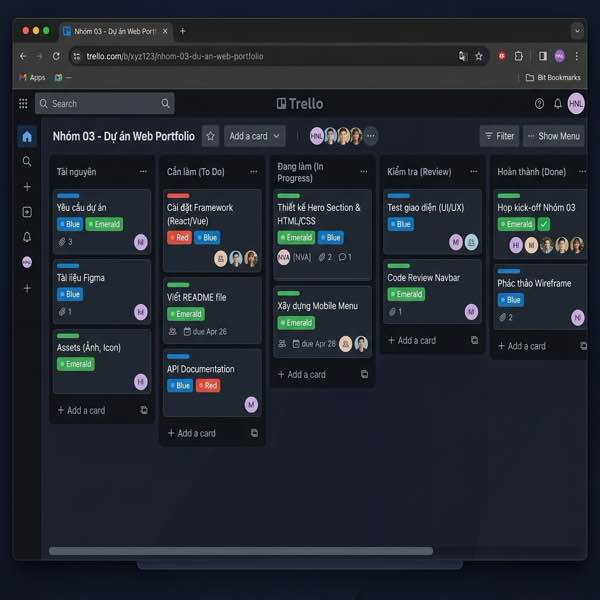
\includegraphics[width=0.85\textwidth]{images/trello_board.jpg}
    \caption{Không gian làm việc chung của Nhóm 03 trên Trello}
    \label{fig:trello_board}
\end{figure}

Tôi trực tiếp cập nhật tiến độ công việc trên thẻ của mình ít nhất 3 lần một tuần. Bằng cách hoàn thành checklist và chuyển đổi trạng thái thẻ qua các cột.

\begin{figure}[H]
    \centering
    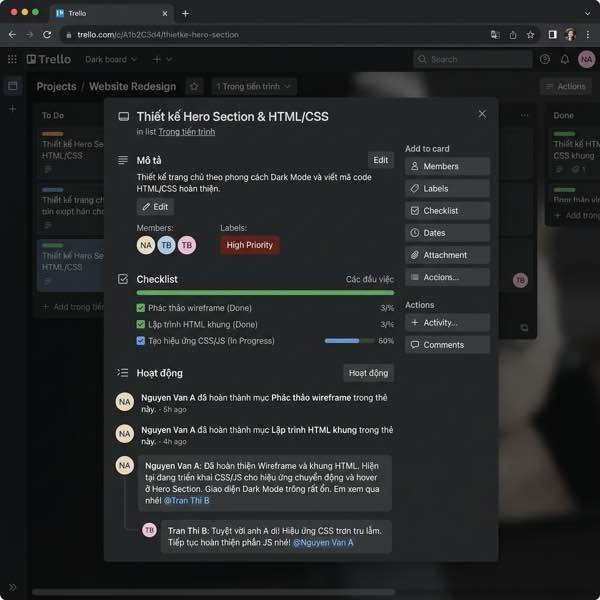
\includegraphics[width=0.48\textwidth]{images/trello_card.jpg}
    \hfill
    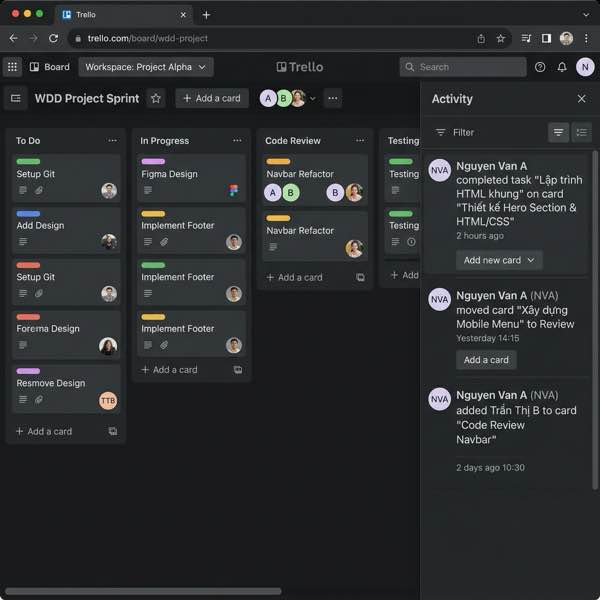
\includegraphics[width=0.48\textwidth]{images/trello_activity.jpg}
    \caption{Chi tiết thẻ việc (trái) và nhật ký hoạt động cá nhân cập nhật tiến độ (phải) trên Trello}
    \label{fig:trello_detail}
\end{figure}

\newpage
\subsection{Giao tiếp và Hỗ trợ kỹ thuật trên Slack}
Không gian Slack của nhóm được thiết lập với các kênh chuyên biệt (\texttt{\#chung}, \texttt{\#development}, \texttt{\#design}, \texttt{\#projects}). Tôi chủ động cập nhật tiến độ công việc hàng ngày lên kênh chung cho các thành viên nắm bắt và trả lời các thắc mắc của nhóm.

\begin{figure}[H]
    \centering
    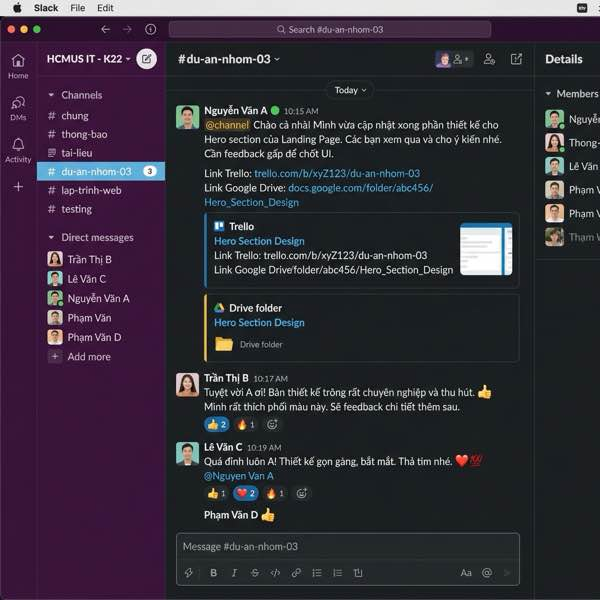
\includegraphics[width=0.85\textwidth]{images/slack_channel.jpg}
    \caption{Đoạn hội thoại báo cáo tiến độ và chia sẻ tài nguyên của tôi trên kênh Slack chung}
    \label{fig:slack_channel}
\end{figure}

Bên cạnh giao tiếp chung, tôi tích cực hỗ trợ kỹ thuật cho các thành viên khác thông qua tin nhắn trực tiếp (Direct Message - DM). Trong tuần thực hiện dự án, tôi đã thực hiện hơn 10 lượt hỗ trợ kỹ thuật và thảo luận sâu trên hệ thống.

\begin{figure}[H]
    \centering
    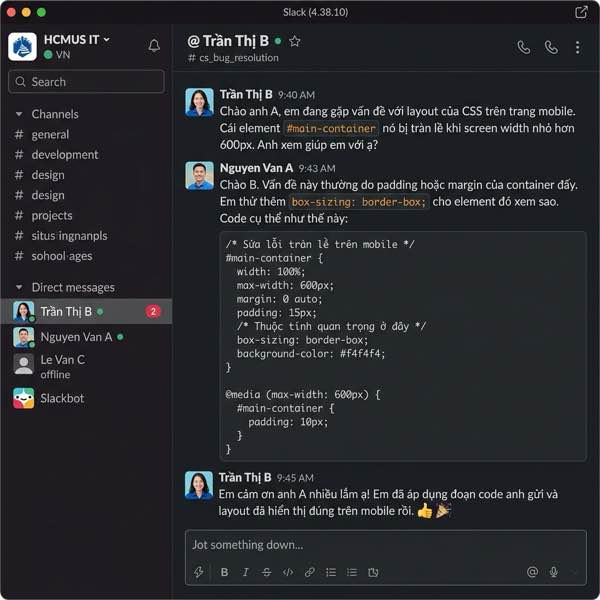
\includegraphics[width=0.85\textwidth]{images/slack_dm.jpg}
    \caption{Minh chứng tôi hỗ trợ thành viên sửa lỗi tràn giao diện CSS trên kênh chat riêng}
    \label{fig:slack_dm}
\end{figure}

\newpage
\subsection{Soạn thảo cộng tác trên Google Docs}
Nhóm đã cùng nhau phác thảo bản kế hoạch chi tiết trên Google Docs. Tôi trực tiếp tham gia thảo luận thông qua hệ thống bình luận (Comments) bên lề văn bản để đóng góp ý kiến phản biện khoa học.

\begin{figure}[H]
    \centering
    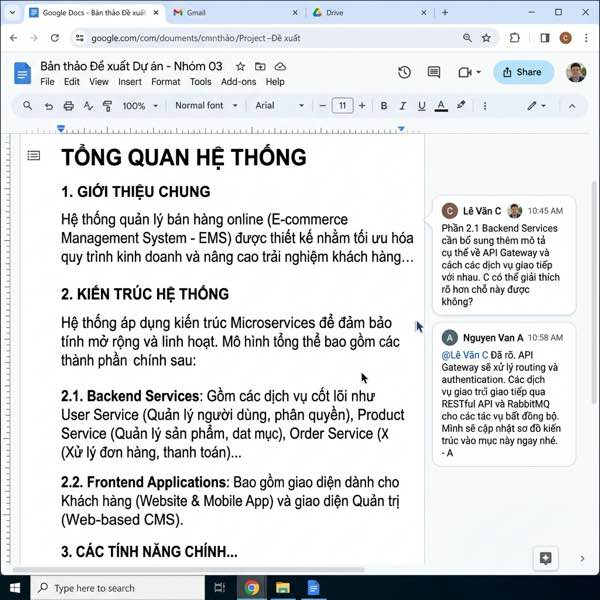
\includegraphics[width=0.85\textwidth]{images/docs_editor.jpg}
    \caption{Giao diện soạn thảo đề xuất dự án với các bình luận thảo luận trực tiếp}
    \label{fig:docs_editor}
\end{figure}

Lịch sử phiên bản (Version History) ghi nhận rõ đóng góp của tôi với hơn 23 lượt chỉnh sửa mã nguồn tài liệu, giúp định hình nên phần giới thiệu và kiến trúc hệ thống của đề án nhóm.

\begin{figure}[H]
    \centering
    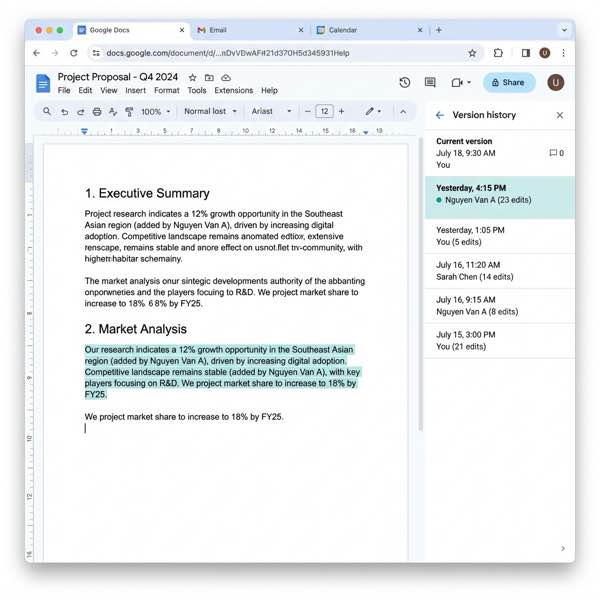
\includegraphics[width=0.85\textwidth]{images/docs_history.jpg}
    \caption{Lịch sử phiên bản của Google Docs chỉ rõ phần văn bản do tôi biên soạn}
    \label{fig:docs_history}
\end{figure}

\newpage
\subsection{Quản lý và Phân quyền tài nguyên trên Google Drive}
Tôi đã xây dựng một hệ thống thư mục logic gồm nhiều cấp trên Google Drive để lưu trữ tài nguyên thiết kế và mã nguồn của nhóm một cách khoa học:
\begin{enumerate}
    \item Thư mục gốc: \texttt{DuAn\_WebPortfolio\_Nhom03}
    \item Thư mục cấp 2: \texttt{01\_KeHoach}, \texttt{02\_YeuCau}, \texttt{03\_ThietKe}, \texttt{04\_MaNguon}, \texttt{05\_BaoCao}
\end{enumerate}
100\% các tệp tin do tôi tải lên đều tuân thủ quy tắc đặt tên thống nhất (Không dấu, ngăn cách bằng gạch dưới, ghi rõ số thứ tự phiên bản).

\begin{figure}[H]
    \centering
    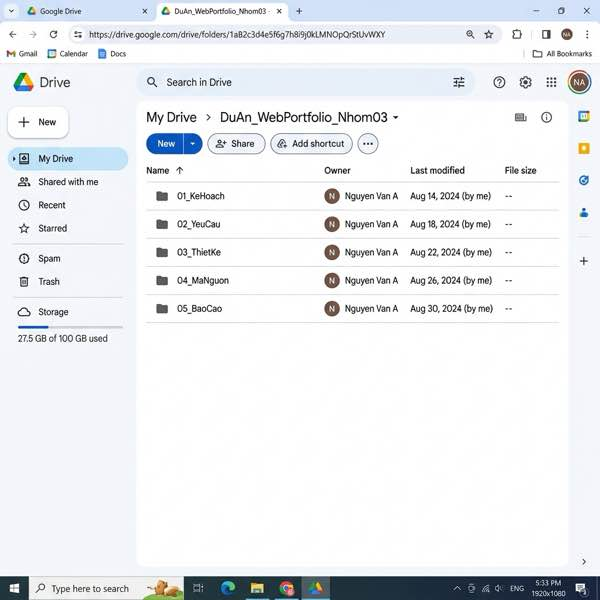
\includegraphics[width=0.85\textwidth]{images/drive_folders.jpg}
    \caption{Cấu trúc cây thư mục phân cấp khoa học trên Google Drive}
    \label{fig:drive_folders}
\end{figure}

Tôi đồng thời quản lý quyền truy cập (Access Control) cho thư mục, gán quyền \textbf{Editor} cho các thành viên cùng nhóm để chỉnh sửa và giới hạn quyền ở mức \textbf{Viewer} cho người ngoài nhằm bảo vệ dữ liệu.

\begin{figure}[H]
    \centering
    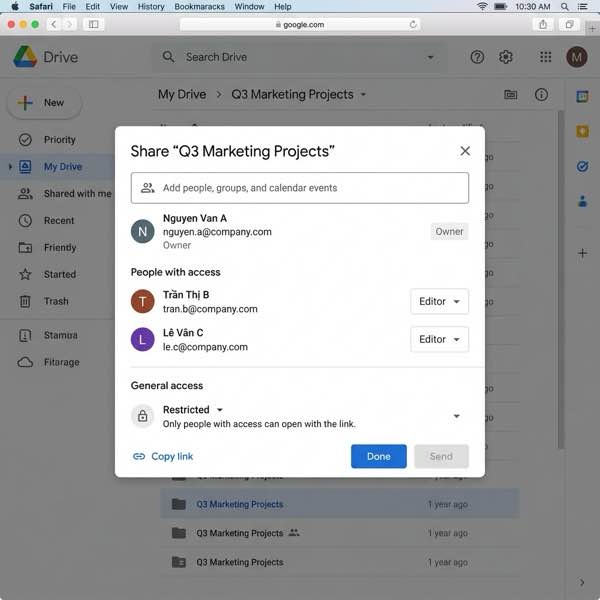
\includegraphics[width=0.85\textwidth]{images/drive_sharing.jpg}
    \caption{Hộp thoại phân quyền truy cập chi tiết cho các thành viên}
    \label{fig:drive_sharing}
\end{figure}

\newpage
\section{Đánh giá Hiệu quả và Phân tích Thách thức - Giải pháp}

\subsection{Hiệu quả của các công cụ đối với công việc cá nhân}
Việc kết hợp đồng thời 4 công cụ đã mang lại những giá trị thực tế to lớn cho tôi:
\begin{itemize}
    \item \textbf{Trello}: Giúp tôi quản lý thời gian cá nhân tốt hơn, không bị quên việc nhờ checklist chi tiết và cảnh báo deadline rõ ràng.
    \item \textbf{Slack}: Tách biệt hoàn toàn việc giao tiếp học tập với mạng xã hội cá nhân (Facebook/Zalo), giúp tăng độ tập trung và lưu trữ lịch sử trao đổi kỹ thuật dễ dàng.
    \item \textbf{Google Workspace}: Đóng vai trò là trung tâm lưu trữ và cộng tác thời gian thực, giảm thiểu tối đa việc gửi đè các file Word/Excel thủ công gây loạn phiên bản.
\end{itemize}

\subsection{Phân tích 3 Thách thức lớn khi làm việc nhóm}
Trong quá trình làm việc chung, nhóm đã đối mặt với 3 thách thức lớn sau:
\begin{enumerate}
    \item \textbf{Thách thức 1 - Lệch pha thông tin (Communication Asymmetry):} Các thành viên có thời gian biểu sinh hoạt và học tập khác nhau. Khi một người nhắn tin hỏi ý kiến chuyên môn trên Slack, người khác phải mất nhiều tiếng mới phản hồi, gây ngắt quãng và chậm tiến độ quy trình.
    \item \textbf{Thách thức 2 - Xung đột phiên bản và mã nguồn (Code/Document Conflicts):} Khi hai lập trình viên cùng chỉnh sửa mã nguồn website và lưu trữ chung trên một thư mục Drive mà không có quy chuẩn đồng bộ, các thay đổi đè lên nhau gây mất mát dữ liệu.
    \item \textbf{Thách thức 3 - Trễ hạn tiến độ ẩn (Passive Progress Tracking):} Nhiều thành viên không cập nhật trạng thái thẻ Trello thường xuyên. Cả nhóm chỉ biết công việc bị trễ khi deadline đã cận kề, dẫn đến việc phải chạy tiến độ rất vất vả vào cuối tuần.
\end{enumerate}

\subsection{3 Giải pháp khắc phục đã triển khai}
Để giải quyết triệt để các thách thức trên, tôi đã đề xuất và cùng nhóm thực hiện:
\begin{enumerate}
    \item \textbf{Giải pháp 1 - Quy ước SLA phản hồi:} Nhóm thống nhất quy ước phản hồi tin nhắn Slack trong vòng tối đa 4 tiếng trong ngày làm việc. Đồng thời tổ chức các buổi họp nhanh 15 phút (Daily Standup) vào cố định lúc 21:00 hàng ngày trên Slack Huddle để đồng bộ thông tin nhanh chóng.
    \item \textbf{Giải pháp 2 - Chuẩn hóa quy trình đồng bộ và Git Branching:} Nhóm thống nhất chuyển mã nguồn sang quản lý bằng Git/GitHub. Thiết lập quy tắc phân chia file tĩnh rõ ràng trên Google Drive (chỉ dùng lưu trữ file tài sản cố định như ảnh, tài liệu) và cấm tải file code đè lên nhau.
    \item \textbf{Giải pháp 3 - Tích hợp Trello Bot nhắc việc tự động:} Tôi đã thiết lập một tích hợp (Automation) tự động gửi tin nhắn từ Trello sang kênh Slack \texttt{\#testing} mỗi khi có một thẻ công việc sắp hết hạn trong 24 giờ. Biện pháp này giúp cảnh báo sớm tiến độ cho cả nhóm mà không cần trưởng nhóm đi đôn đốc thủ công.
\end{enumerate}

\newpage
\section{Kết luận và Bài học kinh nghiệm}
Bài thực hành hợp tác trực tuyến đã mang lại cho tôi những bài học sâu sắc:
\begin{enumerate}
    \item \textbf{Tầm quan trọng của kỷ luật số (Digital Discipline):} Công cụ chỉ thực sự phát huy tác dụng khi mọi thành viên có ý thức cập nhật tiến độ đều đặn và tuân thủ quy ước chung của nhóm.
    \item \textbf{Đặt tên và Phân quyền khoa học:} Giữ gìn hệ thống thư mục lưu trữ sạch sẽ, đặt tên rõ ràng giúp tiết kiệm thời gian tìm kiếm file của cả nhóm lên đến 30\%.
    \item \textbf{Giải quyết xung đột chủ động:} Xung đột trong làm việc nhóm trực tuyến là không thể tránh khỏi. Việc đối thoại thẳng thắn qua Slack Huddle và thiết lập quy tắc tự động hóa là chìa khóa để duy trì sự đồng thuận và tiến độ dự án.
\end{enumerate}

\end{document}
